\documentclass[11pt]{article}

\usepackage[margin=1in]{geometry}
\usepackage{amsmath,amssymb,amsthm}
\usepackage{booktabs}
\usepackage{array}
\usepackage{tikz}
\usetikzlibrary{arrows.meta,positioning}
\usepackage{algorithm}
\usepackage{algpseudocode}
\usepackage{xcolor}
\usepackage{pifont}
\usepackage[colorlinks=true,linkcolor=blue,citecolor=blue,urlcolor=blue]{hyperref}
\usepackage{enumitem}

\newtheorem{proposition}{Proposition}
\newcommand{\code}[1]{\texttt{#1}}
\setlength{\emergencystretch}{3em}  % absorb long \texttt tokens instead of overflowing

\title{\textbf{Correctness Under Time:} \\ Bi-Temporal, Supersession-Aware Memory for AI Agents}
\author{Mayank Sahu \\ \small Independent Researcher \\ \small System: \textsc{Continuum} (open-source; \code{continuum-mcp} on PyPI)}
\date{\today}

\begin{document}
\maketitle

\begin{abstract}
LLM agents do not persist. They forget across sessions, and within a growing memory they surface
stale facts as if current. We present \textsc{Continuum}, a tiered (short/mid/long-term) memory
system whose long-term store is \emph{bi-temporal}: every fact carries a valid-time (when it held
in the world) and a transaction-time (when the system learned it). Supersession is soft. A newer
fact retires the one it contradicts in place, so retrieval stays current while history stays
intact and auditable.

On scripted knowledge-update and point-in-time (``as-of'') benchmarks, \textsc{Continuum} answers
100\% correctly, against 38\% for an append-only store and 20\%/75\% for single-axis (recency,
chronological) baselines. We also run the real Mem0 SDK on the same scenarios. Mem0 resolves
contradictions by deleting the superseded fact and has no valid-time axis. It is competitive at
returning the latest value (72\%) but scores 27\% on point-in-time queries and 30\% on the
bi-temporal set, against \textsc{Continuum}'s 100\%. The gap is structural, not a matter of tuning:
deleting a fact destroys the history an as-of query needs.

On LongMemEval-S \textsc{Continuum} reaches about 74\% judged accuracy. A controlled decomposition
finds the ceiling on that benchmark is answerer reasoning, not retrieval recall; a reasoning loop
we built was net-negative and removed. On BEAM, presenting retrieved memory in chronological rather
than relevance order raises contradiction resolution by 25 points under BEAM's rubric judge, though
\textsc{Continuum} does not out-score Mem0 there. \textsc{Continuum} is open-source, hybrid (bge-m3
+ BM25 fused with RRF over an HNSW-indexed pgvector store), and MCP-exposed. We release the code,
the server, and the benchmark sets.
\end{abstract}

\section{Introduction}

Long-term memory for LLM agents is usually framed as a \emph{retrieval} problem: store past
interactions, embed them, and fetch the top-$k$ most similar passages at query time. This framing
conflates two failure modes that are, in fact, distinct:
\begin{itemize}[leftmargin=1.4em]
  \item \textbf{(a) Knowledge-update.} A fact changes (``I moved from Boston to Seattle''). The old
  fact remains retrievable, so the agent answers with stale information. Recall is not the
  problem: the stale fact is retrieved \emph{correctly}; nothing marks it as retired.
  \item \textbf{(b) As-of / point-in-time.} ``Where did I live in 2021?'' requires reconstructing
  what was true \emph{at a past time}, not what is true now. A store with a single time axis cannot
  answer this; a store with no time axis cannot even represent the question.
\end{itemize}
Vector stores and flat/recency memories get both wrong, and a single end-to-end score hides (b)
entirely. \textsc{Continuum} treats memory as a correctness-under-time problem rather than a
similarity problem. Our contributions are: (1) a bi-temporal, supersession-aware long-term store
that makes knowledge-update and as-of queries \emph{deterministically} correct, with no LLM in the
critical path; (2) released benchmark sets for knowledge-update and as-of queries, with defined
baselines and a run of the real Mem0 SDK on the same scenarios; (3) a retrieval-vs-reasoning
decomposition on LongMemEval, including a reasoning enhancement we removed for being net-negative;
and (4) a production, MCP-exposed open-source system.

\paragraph{Why correctness, not recall.} Consider a long-lived assistant where memory is
correctness-sensitive: a customer agent that must not quote a stale address, or one asked ``what
was true at the time'' for an audit. Here a memory error is a wrong answer with consequences, and a
confidently wrong one, because the stale fact is retrieved perfectly. A guarantee that the current
value is returned without a model guessing is then worth more than a few points of end-to-end
accuracy. This is the regime \textsc{Continuum} targets. We claim the \emph{design} is aimed at
this regime. We do not claim the current single-writer, self-hosted implementation is a drop-in for
a regulated deployment; scale, multi-tenancy, and compliance hardening are out of scope here.

\section{Related Work}

\paragraph{Agent-memory systems.} Mem0~\cite{mem0} performs LLM-based fact extraction
(add/update/delete) with multi-signal retrieval; MemGPT/Letta~\cite{memgpt} treat context as a
virtual memory hierarchy paged by the model; A-Mem~\cite{amem} builds an evolving, self-linking
note store. All optimize \emph{what to store and retrieve} and delegate contradiction handling to
an LLM. \textsc{Continuum} differs in \emph{where} the guarantee lives: correctness under
contradiction and time is a property of the store's bi-temporal schema and deterministic
\code{current()}/\code{timeline()} operators, not of an extraction model. Concretely, none of these
systems carries a \emph{transaction-time} axis, so by Proposition~\ref{prop:retro} they cannot
represent a retroactive correction. We stated this as a falsifiable prediction and tested it
directly (\S\ref{sec:results}): prediction confirmed.

\paragraph{Retrieval-augmented generation.} Dense retrieval + generation~\cite{rag} and hybrid
variants---Reciprocal Rank Fusion~\cite{rrf} over dense (e.g.\ bge-m3~\cite{bgem3}) and
BM25~\cite{bm25} channels on ANN indices such as HNSW~\cite{hnsw}---target recall on a fixed
corpus. \textsc{Continuum} uses this stack for its \code{recall} path but does not rely on it for
correctness; our own ablation finds the hybrid channel statistically indistinguishable from pure
cosine on a semantic needle set (\S\ref{sec:results}), reported as a null.

\paragraph{Temporal data management.} Separating \emph{valid time} from \emph{transaction time} is
long-established in databases~\cite{snodgrass} and standardized as system-/application-time tables
in SQL:2011. Our contribution is not the temporal model but \emph{bringing it to LLM-agent memory}:
exposing bi-temporal \code{current}/\code{timeline} as agent tools over unstructured conversational
facts, where prior agent-memory work uses at most a single clock.

\paragraph{Benchmarks.} LongMemEval~\cite{longmemeval} and LOCOMO~\cite{locomo} measure end-to-end
long-term QA; BEAM~\cite{beam} adds rubric-scored categories. A single end-to-end score conflates
retrieval, reasoning, and the correctness-under-time failure modes we isolate. We use LongMemEval-S
as the primary end-to-end benchmark, add scripted supersession/as-of sets, and report BEAM as a
measured comparison point (\S\ref{sec:beam}) rather than a headline.

\section{System}

\subsection{Tiered architecture}
\textsc{Continuum} organizes memory in three tiers: STM (session-scoped), MTM (consolidated
mid-term), and LTM (durable long-term). Consolidation promotes salient content upward; the LTM tier
holds the bi-temporal guarantees.

\subsection{Formal model}\label{sec:formal}
A \textbf{fact} is a tuple
\[
  f = \big\langle\, s,\; a,\; v,\; [v^-, v^+),\; [t^-, t^+) \,\big\rangle,
\]
where $s$ is the subject, $a$ the attribute, $v$ the value, $[v^-,v^+)$ the \emph{valid-time}
interval ($v^+=\infty$ denotes ``still true''), and $[t^-,t^+)$ the \emph{transaction-time}
interval ($t^+=\infty$ denotes ``not yet invalidated''). The store $S$ is a set of such facts; a
fact is \emph{live} at transaction time $\tau_t$ iff $\tau_t \in [t^-, t^+)$. Supersession is
\emph{soft}: when a newer fact contradicts an older one on the same $(s,a)$, the older fact's
interval is closed; nothing is deleted.

\paragraph{Point-in-time query.} For valid time $\tau_v$ and transaction time $\tau_t$ (both default
to \emph{now}):
\[
  \code{current}(s,a;\tau_v,\tau_t) = v(f^\star), \quad
  f^\star = \operatorname*{arg\,max}_{f \in S}\; v^-(f)
\]
subject to $s(f){=}s,\ a(f){=}a,\ \tau_v \in [v^-,v^+),\ \tau_t \in [t^-,t^+)$: among facts for
$(s,a)$ whose valid interval contains $\tau_v$ and that were believed at $\tau_t$, return the one
with the latest valid-from. \code{timeline}$(s,a)$ returns all such facts ordered by $v^-$. Both are
pure index lookups, with no embedding, ranking, or LLM.

\begin{algorithm}[t]
\caption{Deterministic supersession on write (no LLM)}\label{alg:super}
\begin{algorithmic}[1]
\Procedure{Add}{$f_{\text{new}} = \langle s,a,v_{\text{new}},[v^-_{\text{new}},\infty),[\text{now},\infty)\rangle$}
  \ForAll{$f_{\text{old}} \in S$ with $s(f_{\text{old}}){=}s,\ a(f_{\text{old}}){=}a,\ v^+(f_{\text{old}}){=}\infty$}
    \If{$v^-(f_{\text{old}}) < v^-_{\text{new}}$}
      \State $v^+(f_{\text{old}}) \gets v^-_{\text{new}}$ \Comment{close prior valid interval}
    \Else
      \State keep both; older fact wins valid-time, history retained
    \EndIf
  \EndFor
  \State insert $f_{\text{new}}$
\EndProcedure
\end{algorithmic}
\end{algorithm}

The $(s,a)$ key makes Algorithm~\ref{alg:super} decidable \emph{without} an LLM. Generalizing it
from tagged writes to open conversation text---deriving $(s,a)$ for untagged facts---is engineering
that widens coverage; the guarantee is unchanged.

\begin{proposition}\label{prop:retro}
A correction may carry a valid-from \emph{earlier} than the fact it supersedes. Any store that
orders facts by a single clock ranks such a correction as stale.
\end{proposition}

\emph{Instance (from the shipped store).} At $\tau_1$ the user asserts ``I live in Lisbon''
($v^-=\tau_1$). At $\tau_2 > \tau_1$ the user says ``I moved to Porto on July~1'' with
$\text{Jul 1} < \tau_1$ ($v^-=\text{Jul 1}$, learned at $\tau_2$). Ordering by valid-time alone
makes \emph{Lisbon} look newer than the \emph{Porto} correction, so a single valid-axis store
answers ``Lisbon,'' which is wrong. Transaction time disambiguates: Porto was believed later, so it
supersedes (Figure~\ref{fig:bitemporal}). This is exactly the \code{naive\_chronological} failure
measured in \S\ref{sec:results} (point-in-time 100\%, retroactive 0/5); the bi-temporal split
recovers all five.

\begin{figure}[t]
\centering
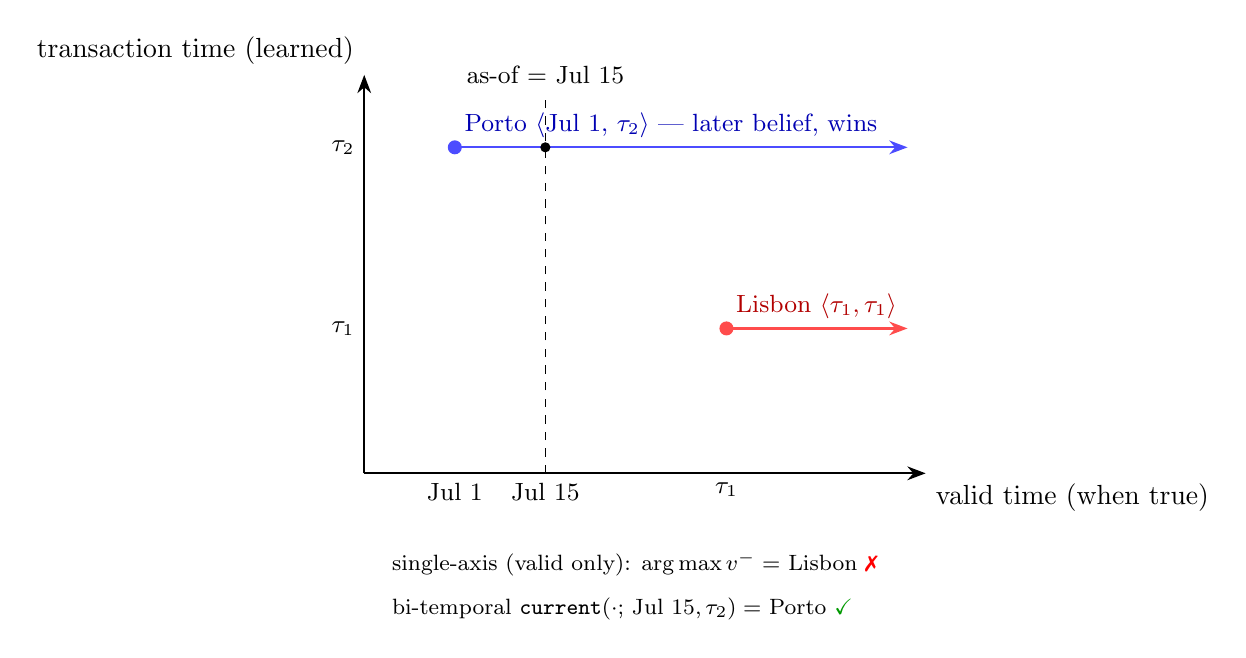
\begin{tikzpicture}[>=Stealth, scale=1.15]
  % axes
  \draw[->,thick] (0,0) -- (6.2,0) node[below right] {valid time (when true)};
  \draw[->,thick] (0,0) -- (0,4.4) node[above left] {transaction time (learned)};
  % ticks
  \node[below] at (1,0) {\small Jul 1};
  \node[below] at (2,0) {\small Jul 15};
  \node[below] at (4,0) {\small $\tau_1$};
  \node[left] at (0,1.6) {\small $\tau_1$};
  \node[left] at (0,3.6) {\small $\tau_2$};
  % valid half-lines
  \draw[blue!70,thick,->] (1,3.6) -- (6.0,3.6);
  \draw[red!70,thick,->]  (4,1.6) -- (6.0,1.6);
  % points
  \fill[blue!70] (1,3.6) circle (2.2pt) node[above right,blue!70!black] {\small Porto $\langle$Jul 1, $\tau_2\rangle$ — later belief, wins};
  \fill[red!70]  (4,1.6) circle (2.2pt) node[above right,red!70!black] {\small Lisbon $\langle\tau_1,\tau_1\rangle$};
  % query line
  \draw[dashed] (2,0) -- (2,4.2) node[above] {\small as-of $=$ Jul 15};
  \fill (2,3.6) circle (1.6pt);
  % verdict (two explicit lines so they never run off the right margin)
  \node[anchor=west,font=\footnotesize] at (0.2,-1.0)
    {single-axis (valid only): $\arg\max v^- =$ Lisbon~\textcolor{red}{\ding{55}}};
  \node[anchor=west,font=\footnotesize] at (0.2,-1.5)
    {bi-temporal \code{current}$(\cdot;\,\text{Jul 15},\tau_2) =$ Porto~\textcolor{green!60!black}{$\checkmark$}};
\end{tikzpicture}
\caption{The two-axis view of the retroactive example. The query at valid time Jul~15 meets Porto's
valid half-line $[\text{Jul 1},\infty)$ but not Lisbon's $[\tau_1,\infty)$; the transaction axis
identifies Porto as the later belief. A single valid-time axis answers wrongly.}
\label{fig:bitemporal}
\end{figure}

\subsection{Hybrid retrieval and MCP surface}
The \code{recall} path is hybrid: dense (bge-m3, 1024-d) and BM25 fused with RRF over an
HNSW-indexed (\code{halfvec\_cosine\_ops}) pgvector store. Retrieval is relevance-ranked and must
\emph{filter} superseded facts, whereas \code{current}/\code{timeline} are exact. \textsc{Continuum}
exposes four MCP tools (\code{remember}, \code{recall}, \code{current}, \code{timeline}), shipped
as \code{continuum-mcp}, making the deterministic operators directly available to any MCP-capable
agent.

\section{Evaluation Setup}

\textbf{Datasets.} (i) LongMemEval-S (500 questions, LLM-judged). (ii) A scripted
\textbf{supersession} set of 50 knowledge-update scenarios across 6 attribute types. (iii) A
scripted \textbf{bi-temporal as-of} set of 20 timelines (15 point-in-time, 5 retroactive corrections).

\textbf{Determinism.} All supersession and as-of numbers use the LLM supersession decider
\emph{disabled}: they exercise only the deterministic exact-tag + valid-time path
(\code{bench/supersession\_e2e.py} runs with no API key).

\textbf{Mem0 comparison.} The real Mem0 SDK (v0.1.67) is configured fully locally: a HuggingFace
\code{all-MiniLM-L6-v2} embedder, a Chroma vector store, and gpt-4o-mini for Mem0's internal
extraction/update and for the answer step, with a fresh \code{user\_id} per scenario. Statements
are ingested in learned (transaction-time) order; the query is answered over Mem0's retrieved
memories and scored against the same ground truth (\code{bench/mem0\_compare.py}).

\section{Results}\label{sec:results}

\begin{table}[t]
\centering\small
\begin{tabular}{@{}p{5.0cm}p{4.3cm}p{4.6cm}@{}}
\toprule
\textbf{Result} & \textbf{\textsc{Continuum}} & \textbf{Baseline(s)} \\
\midrule
Supersession, in-memory sim (50) & \textbf{100\%} (50/50) & \code{naive\_append} \textbf{38\%} (19/50) \\
Supersession, end-to-end / Postgres, no LLM (50) & \code{current()} \textbf{100\%} $\cdot$ \code{recall} top-1 \textbf{20\%} & \textbf{Mem0} (real SDK) \textbf{72\%} (36/50) \\
Bi-temporal ``as-of'' (20 = 15 PIT + 5 retro) & \textbf{100\%} (20/20) & \code{naive\_latest} \textbf{20\%} $\cdot$ \code{naive\_chrono} \textbf{75\%} (retro 0/5) $\cdot$ \textbf{Mem0 30\%} (PIT 4/15, retro 2/5) \\
LongMemEval-S (500, judged, gpt-oss-120b) & \textbf{$\sim$74\%} & 60.8\% v1.0 $\cdot$ 34.4\% earlier ceiling \\
Retrieval decay R@10 (3k/25k/47k) & \textbf{1.00 / .90 / .85} & pgvector-cosine (ties, below) \\
Hybrid vs.\ cosine (MRR) & .916 / .900 / .800 & .916 / .903 / .750 (within noise) \\
\bottomrule
\end{tabular}
\caption{Main results. Correctness-under-time numbers use no LLM in the critical path.}
\label{tab:main}
\end{table}

\paragraph{The two-axis argument.} \code{naive\_chronological} (a single valid-time axis) gets
point-in-time queries 100\% right yet 0/5 on retroactive corrections: a fact learned late about the
past is invisible to a one-axis store. Splitting valid- from transaction-time recovers all five,
taking \textsc{Continuum} to 20/20. The result is a consequence of the data model, not of tuning.

\paragraph{End-to-end validation.} Replaying the 50 supersession scenarios through the shipped
\code{Memory.from\_postgres} path gives \code{current()} 100\% (50/50, 0 stale) with no LLM and no
API key. Through the same path \code{recall} top-1 is only 20\%. This shows where the LLM matters:
the decider is needed only to keep the relevance-ranked \code{recall} path from surfacing stale
facts, not for \code{current}/\code{timeline} correctness.

\paragraph{Head-to-head with Mem0.} We ran the real Mem0 SDK on the same scenarios. On returning
the current value, Mem0's LLM-driven update reaches 72\% (36/50). That beats \textsc{Continuum}'s
un-decidered \code{recall} path (20\%), though it trails the deterministic \code{current()} (100\%).
On ``what was true \emph{then}'', Mem0 fails: 4/15 (27\%) point-in-time, 2/5 retroactive, 30\%
overall, against \textsc{Continuum}'s 100\%. The store shows why. For ``where did the user live in
mid-2024?'' (answer: Boston), Mem0's entire memory was \texttt{['Relocated to Austin last week']}:
the Boston and NYC facts had been deleted by its update operation, so it answered \emph{UNKNOWN}.
Where it retained both facts, it answered the wrong era (\emph{Portland} for a late-2022 query),
having no valid-time axis to select on. This confirms Proposition~\ref{prop:retro}. A system that
resolves contradictions by overwriting cannot answer as-of queries, because the overwrite destroys
the history the query needs.

\paragraph{Hybrid vs.\ cosine.} Across 3k/25k/47k the shipped hybrid and a plain pgvector cosine
scan are statistically indistinguishable (every gap is a single needle out of 20, within HNSW build
noise). We do not claim hybrid beats cosine on this semantic set; the claim is $\ge$, no worse. The
lexical channel's contribution would have to be shown on an exact-match query set, which we leave to
future work.

\section{The Retrieval-vs-Reasoning Decomposition}

Seven sweeps across four model families and six retrievers found a hard $\sim$32--34\% substring
ceiling \emph{even at 100\% recall}, localizing the bottleneck to multi-hop reasoning in the
answerer. What moved the end-to-end number was a stronger answerer over direct retrieval with judged
scoring (60.8\% to about 74\%). A reasoning loop we predicted we would need was built, A/B-tested,
and cut as net-negative. That is the empirical core of the ``retrieval is not the ceiling'' claim.

\section{Presentation Order, and a Negative BEAM Result}\label{sec:beam}

BEAM scores categories with per-question rubric nuggets (each judged 0/0.5/1.0; a question passes
at mean $\ge 0.5$). Presentation order matters here. On BEAM-100K (gpt-oss-120b answerer, rubric
judge), presenting the top-$k$ retrieved turns in chronological rather than relevance order lifts
contradiction resolution from 7.5\% to 32.5\% (+25pp) and nudges event ordering 27.5\% to 32.5\%;
time-ordering surfaces both sides of a contradiction. \textsc{Continuum} does not out-score Mem0 on
BEAM. Mem0's published numbers (48.6\% / 60.0\%) use a gpt-5 answerer and judge on the 1M split;
ours use an open answerer on the 100K split, and the rubric rewards verbose both-sides answers, so
the score reflects answer style as much as memory quality. We treat BEAM as a comparison point
rather than a headline.

\section{Limitations}

\begin{itemize}[leftmargin=1.4em]
  \item Judged $\sim$74\% on LongMemEval-S is not state-of-the-art; the win is the deterministic
  correctness axes, which are answerer-independent.
  \item \textsc{Continuum}'s un-decidered \code{recall} path (20\%) is weaker than Mem0's LLM-update
  recall (72\%) on returning the current value. The deterministic \code{current()} is 100\%, but the
  relevance-ranked \code{recall} surfaces stale facts unless the optional decider has invalidated
  them. Deterministic, validity-aware \code{recall} that filters superseded facts at the query layer
  is the highest-value engineering item.
  \item The Mem0 comparison uses gpt-4o-mini and a small local embedder; a stronger answerer could
  shift the \emph{latest-value} number but not the point-in-time result, which is bounded by the
  data model (a deleted fact cannot be retrieved at any answerer strength).
  \item Retrieval recall decays with store size (85\% R@10 at $\sim$47k); single-writer
  supersession only; scripted benchmarks are small (50/20) and released for others to extend.
\end{itemize}

\section{Conclusion}

\textsc{Continuum} reframes agent memory from similarity to \emph{correctness under contradiction
and time}. Its bi-temporal, supersession-aware store answers knowledge-update and as-of queries
deterministically (100\% vs 38\%/20\%/75\% baselines, and vs Mem0's 30\% on the bi-temporal set),
while a decomposition shows the residual end-to-end ceiling is answerer reasoning, not retrieval. We release the repository, \code{continuum-mcp}, the harnesses, and the
supersession/bi-temporal benchmark sets with scoring scripts.

\begin{thebibliography}{99}
\small
\bibitem{mem0} Mem0: The Memory Layer for Personalized AI. \url{https://github.com/mem0ai/mem0}, 2024.
\bibitem{memgpt} C.\ Packer et al. MemGPT: Towards LLMs as Operating Systems. \emph{arXiv:2310.08560}, 2023.
\bibitem{amem} A-Mem: Agentic Memory for LLM Agents. \emph{arXiv preprint}, 2025.
\bibitem{rag} P.\ Lewis et al. Retrieval-Augmented Generation for Knowledge-Intensive NLP Tasks. \emph{NeurIPS}, 2020.
\bibitem{rrf} G.\ V.\ Cormack, C.\ L.\ A.\ Clarke, S.\ Buettcher. Reciprocal Rank Fusion. \emph{SIGIR}, 2009.
\bibitem{bgem3} J.\ Chen et al. BGE M3-Embedding: Multi-Lingual, Multi-Functionality, Multi-Granularity. \emph{arXiv:2402.03216}, 2024.
\bibitem{bm25} S.\ Robertson, H.\ Zaragoza. The Probabilistic Relevance Framework: BM25 and Beyond. \emph{FnTIR}, 2009.
\bibitem{hnsw} Y.\ Malkov, D.\ Yashunin. Efficient and Robust ANN Search Using HNSW Graphs. \emph{IEEE TPAMI}, 2018.
\bibitem{snodgrass} R.\ T.\ Snodgrass. \emph{Developing Time-Oriented Database Applications in SQL}. Morgan Kaufmann, 1999.
\bibitem{longmemeval} D.\ Wu et al. LongMemEval: Benchmarking Chat Assistants on Long-Term Interactive Memory. \emph{arXiv:2410.10813}, 2024.
\bibitem{locomo} A.\ Maharana et al. Evaluating Very Long-Term Conversational Memory of LLM Agents (LOCOMO). \emph{ACL}, 2024.
\bibitem{beam} BEAM: A Benchmark for Episodic Agent Memory. HuggingFace dataset \texttt{Mohammadta/BEAM}, 2026.
\end{thebibliography}

\end{document}
